\subsection{Resumen}
Queremos corroborar que el compilardo icc es mejor, en terminos temporales (mas adelante se analizara el comportamiento respecto de la cache), que el compilador gcc.

\subsection{Experimentacion}
Para analizar los compiladores usaremos el filtro diff. Lo aplicaremos sobre cuatro imagenes, de diferente tamaño. Sobre cada imagen, correremos el filtro varias veces, dado que los procesos de nuestra computadora pueden afectar temporalmente a los filtros. De esta manera, nos aproximaremos mas al resultado real. Calcularemos la desviacion estandar, para reflejar que solo es una aproximacion \\
Para cada imagen, la procesamos utilizando ambos compiladores y anotamos los tiempos (en ciclo de clocks), y a estos, los dividimos por la cantidad de pixel de la imagen. Asi, obtenemos cuanto tarda, en promedio, procesar un pixel. Luego, de estos valores, obtenemos la media y la desviacion estandar. Tomaremos el tamaño de la imagen como la cantidad de pixeles, dado que se procesan todos los pixeles en orden consecutivo, con lo cual no habria diferencia si la imagen tuviera otra largo o ancho

\subsection{Resultados}
Hechas las mediciones, obtenemos lo siguiente

\begin{figure}[H]
\begin{center}
\minipage{0.8\textwidth}
  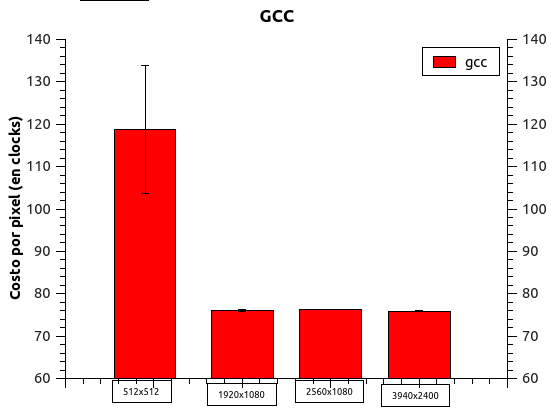
\includegraphics[width=\linewidth]{tiemposCompiladores/gcc.png}
  \caption{{\small Medicion de gcc}} 
\endminipage
\end{center}
\end{figure}

\begin{figure}[H]
\begin{center}
\minipage{0.8\textwidth}
  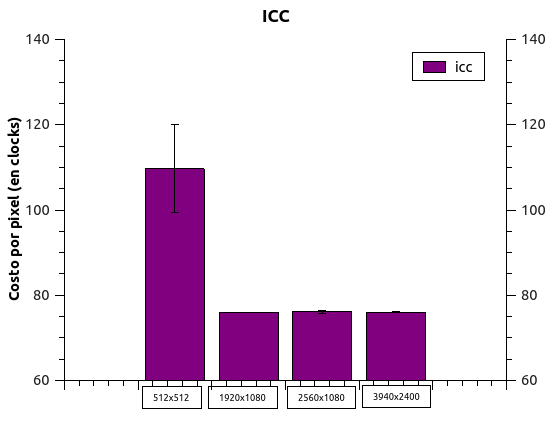
\includegraphics[width=\linewidth]{tiemposCompiladores/icc.png}
  \caption{{\small Medicion de icc}} 
\endminipage
\end{center}
\end{figure}

\begin{figure}[H]
\begin{center}
\minipage{0.8\textwidth}
  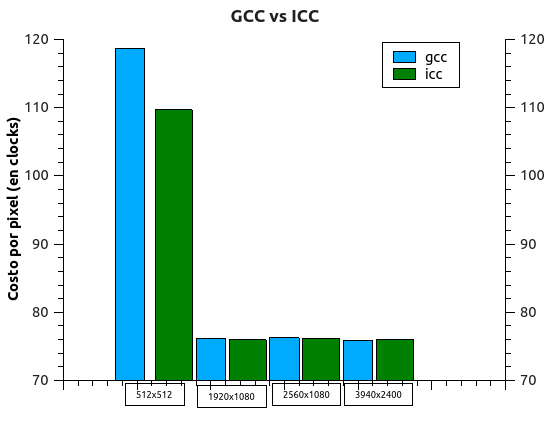
\includegraphics[width=\linewidth]{tiemposCompiladores/gccVsIcc.png}
  \caption{{\small Comparacion entre gcc y icc}} 
\endminipage
\end{center}
\end{figure}

Podemos analizar las siguientes cosas de los resultados obtenidos: \\
Primero, en la imagen mas pequeña, el tiempo de procesamiento por pixel es bastante mayor que en las imagenes mas grandes, en las cuales el tiempo por pixel es casi el mismo. Esto sucede en ambos compiladores. Creemos que esto puede deberse a que hay alguno/algunos procesos en la computadora que no son constantes (es decir, no ocurren cada x cantidad de ciclos) y que influyen en los tiempos. Por eso para imagenes pequeñas se nota su influencia, pero para imagenes grandes no. Tiene sentido entoneces, que la desviacion estandar nos de mucho mas alta en la imagen de menor tamaño
Segundo, si bien para la imagen mas pequeña se puede observar que el compilador icc procesa mas rapido, no existe tal diferencia para las imagenes mas grandes. Incluso, en la imagen mas grande, es mas rapido (aunque la diferencia es cercana al 1$\%$)
\subsection{Conclusion}
Refutamos, tristemente, nuestra hipotesis y concluimos entonces que el compilador icc no tiene ventaja sobre gcc. Compararemos mas adelante el uso de la cache, pero, a priori, no vale la pena gastar plata en icc.
